\documentclass[conference]{IEEEtran}
\IEEEoverridecommandlockouts
% The preceding line is only needed to identify funding in the first footnote. If that is unneeded, please comment it out.
\usepackage{cite}
\usepackage{amsmath,amssymb,amsfonts}
\usepackage{algorithmic}
\usepackage{graphicx}
\usepackage{textcomp}
\usepackage{xcolor}
\makeatletter
\newcommand*{\rom}[1]{\expandafter\@slowromancap\romannumeral #1@}
\def\BibTeX{{\rm B\kern-.05em{\sc i\kern-.025em b}\kern-.08em
    T\kern-.1667em\lower.7ex\hbox{E}\kern-.125emX}}
    %%%%%%%%%%%%%%%%%%%%%%%%%%%%
\makeatletter
%%%%%%%%%%%for copyright notice
\makeatletter
%%%%%%%%%%%for copyright notice
\def\ps@IEEEtitlepagestyle{%
    \def\@oddfoot{\mycopyrightnotice}%
    \def\@evenfoot{}%
}
\def\mycopyrightnotice{%
    {\footnotesize  978-1-7281-7366-5/20/\$31.00 \textcopyright2020 IEEE\hfill}
    \gdef\mycopyrightnotice{}
}
%%%%%%%%%%%
\makeatletter
\newcommand{\algrule}[1][.2pt]{\par\vskip.5\baselineskip\hrule height #1\par\vskip.5\baselineskip}
\makeatother
\makeatletter
\newcommand*\titleheader[1]{\gdef\@titleheader{#1}}
\AtBeginDocument{%
  \let\st@red@title\@title%
  \def\@title{%
    \bgroup\normalfont\normalsize\raggedright\@titleheader\par\egroup
    \vskip1.5em\st@red@title}
}
\makeatother
\title{EMG Controlled Bionic Robotic Arm\\ using Artificial Intelligence and
Machine Learning}
\titleheader{2020 IEEE Region 10 Symposium (TENSYMP), 5-7 June 2020, Dhaka, Bangladesh}
\makeatletter
\newcommand{\linebreakand}{%
  \end{@IEEEauthorhalign}
  \hfill\mbox{}\par
  \mbox{}\hfill\begin{@IEEEauthorhalign}
}
\makeatother

\author{
  \IEEEauthorblockN{\textsuperscript{} Farhan Fuad Rupom}
  \IEEEauthorblockA{\textit{Computer Science and Engineering} \\
    \textit{\textit{BRAC} University}\\
   Dhaka, Bangladesh\\
    rupom.cse16@gmail.com}
  \and
  \IEEEauthorblockN{\textsuperscript{}Shafaitul Jannat}
  \IEEEauthorblockA{\textit{Computer Science and Engineering} \\
   \textit{\textit{BRAC} University}\\
    Dhaka, Bangladesh\\
    shipa96jannat@gmail.com}
  \and
  \IEEEauthorblockN{\textsuperscript{} Farjana Ferdousi Tamanna}
  \IEEEauthorblockA{\textit{Computer Science and Engineering} \\
    \textit{\textit{BRAC} University}\\
    Dhaka, Bangladesh \\
    tamannamou76@gmail.com}
  \linebreakand % <------------- \and with a line-break
  \IEEEauthorblockN{\textsuperscript{} Gazi Musa Al Johan}
  \IEEEauthorblockA{\textit{Computer Science and Engineering} \\
    \textit{\textit{BRAC} University}\\
    Dhaka, Bangladesh \\
    johandipto19@gmail.com}
  \and
  \IEEEauthorblockN{\textsuperscript{} Md. Motaharul Islam}
  \IEEEauthorblockA{\textit{Computer Science and Engineering} \\
    \textit{United International University}\\
    Dhaka, Bangladesh \\
    motahariut@gmail.com}
}
\begin{document}

% Change according to their suggestion


\maketitle
\begin{abstract}
The fundamental and main goal of gesture recognition research applied to Human-Computer
Interaction (HCI) is making systems to identify and classify some specific human gestures and
use them to transfer information and control devices. Surface Electromyography (sEMG) based
gesture interfaces need quick and accurate detection, and gesture recognition in real time. We have mainly worked with four hand gestures which are Rock, Paper, Spherical grip, All right. This report proposes a solution to do real-time gesture recognition with the use of various
machine learning algorithms and allowing its applications in a vast range of human-computer
interfaces. We have used sEMG recordings recorded from muscles of hand which will constantly
transmit those data to microcontroller. We will collect data from the microcontroller and then
store those data in offline server.
\end{abstract}

\begin{IEEEkeywords}
Surface EMG, gesture recognition, machine learning, micro-controller
\end{IEEEkeywords}

\section{Introduction}
Bionic robotic arm is a system where the machine can receive user feedback through an electromyography sensor and can operate according to the user's behavior through an artificial hand or simulation. Electromyography approach along with hybrid algorithm classification improves efficiency of a prosthetic system by employing greater responsiveness and accurate gesture performance. This system is done to improve the experience of an amputee and to minimize production cost to a larger extent. The classification technique implemented through Support Vector Machine (SVM) and K-Nearest Neighbour (KNN) determines the desired gesture of an amputee, this is accomplished using signal filtration along with signal processing and various feature extractions. Conventional gesture detection approaches and performing prosthetic arms are not cost efficient and not faultless. Hence an improved gesture detection and performing approach has been proposed to improve the production cost along with efficiency. The proposed technique presents improved numerical outcome than other conventional systems. A notable recognition methodology and bug fixing strategy are hybrid algorithm technique and simulation. The comparison between single algorithm based system and hybrid algorithm based system were implemented based on outcome percentage where the hybrid system was able to distinguish between the hand gesture classes through activating KNN and SVM algorithm instructions sub-sequentially based on the efficiency of individual algorithms. To make more precise system with lesser cost, the given below ideas are based on our contributions:
\begin{itemize}
   \item The system has mainly focused on the trans-radial prosthesis as it is an artificial limb that replaces an arm missing below the elbow which is called upper limb prosthesis.
   \item Statistical methods has been used to extract and visualize muscular co-activation patterns captured in our recordings. 
   \item EMG classifiers have been built in order to discriminate between different gestures in different positions.
   \item Finally, after identifying different gestures, the results and data can be used to convey information and to control a bionic robotic arm.
\end{itemize}
Unfortunately, many individuals all over the world are losing their arms every day due to injuries or medical complications. In Bangladesh, the proportion of people with disabilities is growing as traffic and workplace accidents like other developing countries. An analysis of the figures reveals  that  2.1 million people have been now losing the arms in various collisions, injuries and illness in United States \cite{abc20}. Around 1,85,000 men are amputated every year \cite{abc23}. This continues to lead to daily 300 to 500 surgeries \cite{abc23}. Any 30\% of people could have a depressive disorder \cite{abc23} for loss of limbs. Health costs for amputees are 509, 275 million \$ which is greater comparing other patients \cite{abc23}. Clinical costs for people amputated in 2013 amounted to \$8.7 billion \cite{abc23}. 55\% among those who have diabetes  undergoes into second limb amputation after the first limb amputation within 2 to 3 years \cite{abc23}. Most of the available prosthetic and systems are costly for most of the amputees. Again low priced  prosthetic  can not perform precisely like those costly system. So that, more amputees around the globe needs affordable prosthetic with precise performance.\\
The rest of the paper has been described in the following manner. Section \rom{1} discusses about the importance about bionic arm. Objectives behind this research has been presented in section \rom{2} and the section \rom{3} describes about the related works. The proposed system architecture has been discussed at the section \rom{4} and theoretical procedures has been described in the section \rom{5} along with the algorithms which are proposed. The implementation of this system is discussed in the section \rom{6}. Section \rom{7} represents the result and analysis. Lastly, section \rom{8} concludes our system.

\section{Research objective}
The objective of this research is to create a system where the data and information of user will be acquired and classified precisely to increase system accuracy with affordability. Most of the budget friendly prosthetic limbs are not able to maintain the synchronization between processing and responsiveness to users information. In the many case, they are not able to perform accurate gestures. On the other hand, prosthetic arms with improved quality in performance, are not affordable for financially back lagged people. For these reasons, the purpose of this research is to develop a system with minimum production cost and also with precised data classification. Another purpose behind the system is to represent the improved accuracy efficiency of hybrid algorithm approach in EMG gesture classification. The motivation is to build a system in which the user can move his prosthetic hands almost like a real bio hand which will be produced with low cost and greater accuracy.

\section{Literature Review}
Johnny L. G. Nielsen et al. \cite{nielsen2010simultaneous}  proposed a novel approach done with surface electromyogram to
record information from one upper limb to force generated using the collateral limb. They measured from the right wrist in multiple degrees of freedom along with different movements. J. Carpaneto et al. \cite{6290769} proposed a prosthetic limb using the EMG signal. EMG-based stimulation is done by machine learning in the nervous system and the use of implantation of
electrodes in the muscles. The vector machine algorithm had been used to predict different types of grip including grasp gestures using both distal and proximal upper limb tissues with EMG
activity. Katsutoshi Kuribayashi et al. \cite{407610} proposed using neural networks to monitor the electromyography and form memory material using two methods. The first one was EMG signal
rectification and integration and the another one was the cycle of the neural network. Because of light weight and compact, SMA was used to compare the EMG signal. In  \cite{abc21} researchers recorded myoelectric responses from two adult macaque monkeys with 12 items of various shapes to distinguish among types of EMG stimulation associated with particular grasping behaviors.

\section{System Architecture}
This system has been structured into an architecture of three-tier where each tier performs a particular logical function located in distinguishable physical devices and all tiers are interconnected. The tiers named EMG Signal Device, Gesture processing and control, Terminal devices is shown in Fig~\ref{fig:flow chart}. EMG signal device is an interface tier operated by a hardware which captures possible signals of different gestures with an efficient speed to ensure valid commands for terminal devices. The tier named Gesture processing and control handles the signal filtering, processing as well as classifying gestures with the help of trained data. It alsos serves the terminal devices with proper command by executing proper code and instructions. After predicting the proper hand gesture, that corresponding gesture gets performed by the Terminal devices tier where simulation or 3d printed model are located. 
\begin{figure}[htbp]
 \centerline{ 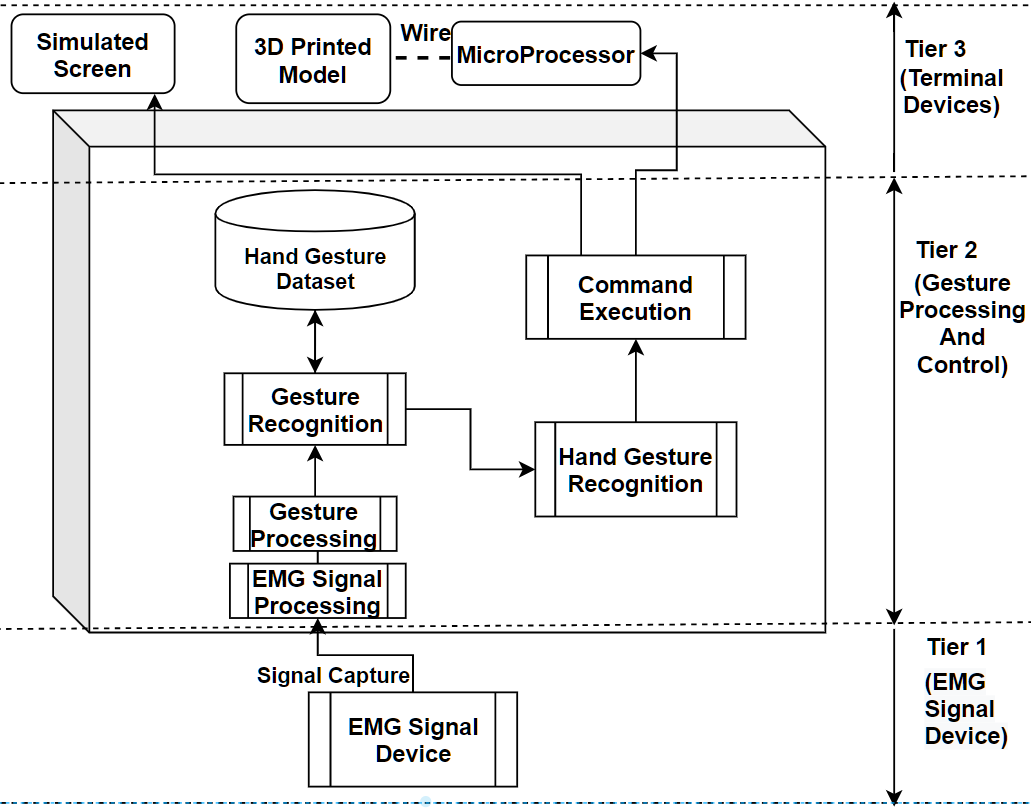
\includegraphics[scale=0.4]{Capture1 (5).PNG}}
  \caption{The proposed system architecture}
  \label{fig:flow chart}
\end{figure}

\section{System Methodology}
In this proposed model, real data has been collected through EMG signal. Then pre-processing and feature extraction of those signals has been  done using different methods. After that, data set has been classified for getting the most accurate value for motion recognition. Finally, those values has been implemented on the system's simulated model in order to asses the accuracy of the system. The whole method has been represented in Fig~\ref{fig:1}.
\begin{figure}[htbp]
\centerline{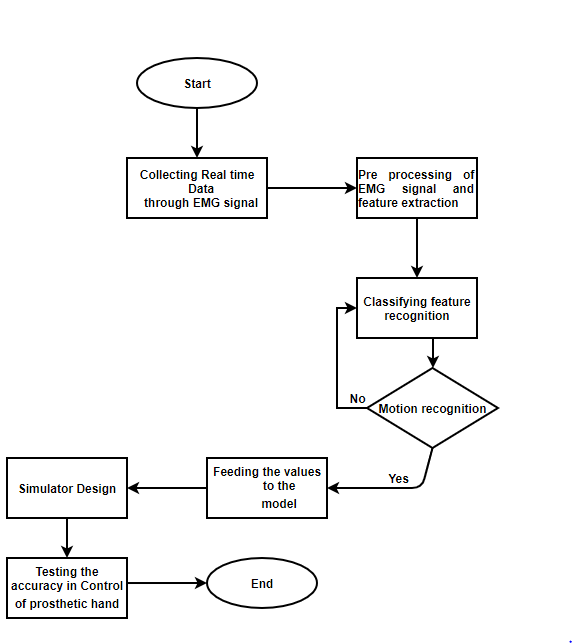
\includegraphics[scale=0.6]{Capturex.PNG}}
\caption{Flowchart of Bionic Robotic arm}
\label{fig:1}
\end{figure}

\subsection{SVM}\label{AA}
A binary classifier, which determines whether or not a sample is in one class, can be described as SVMs. It employs the principle of optimizing structural hazards which compromise the methodological pitfalls and the model's intricacy \cite{10.1023/A:1009715923555}.
\begin{figure}[h!]
\centerline{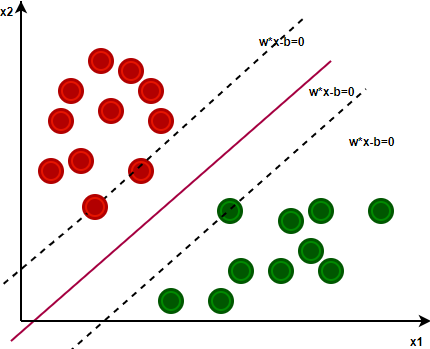
\includegraphics[scale=0.5]{Capturexx (2).PNG}}
  \caption{ Hyper plane with distinguishable data (linear model)}
  \label{fig:graph}
\end{figure}
The construction of a decision surface is an integral part of an SVM, so as to maximize the
distance from positive to negative examples. The judgment surface has a high level, since the numbers of input vector components belongs to $\mathbb{R}^{n}$ (Real Numbers). For linearly separable data, it can be distinguished with an optimal separator line \cite{10.1023/A:1009715923555}. For this, the optimal hyper plane for classification can be described
by \cite{10.1023/A:1009715923555},
\begin{align}
 w^Tx_i+b = 0 
\end{align}
where w is a vector of weight and x a vector of input. The ideal hyper plane with two-dimensional linearly separable information shows an example in Fig~\ref{fig:graph}. A particular set of input vectors is defined for this hyper plane,  known  as  supporting  vectors.  Several input vectors are positioned adjacent to the optimum hyper plane and categorization is then rendered \cite{HsuLibsvmTutorial2003}. According to the following terms for any variable like $x_i$ \cite{HsuLibsvmTutorial2003},
\begin{align}
 w^Tx_i+b \geq 0 \quad \quad   y_i&=y_i+1 \\
 w^Tx_i+b < 0 \quad \quad  y_i&=y_i-1
\end{align}
\
\subsection{KNN}\label{BB}
K-Nearest Neighbor (KNN) plays a significant role in pattern recognition. This method identifies
the homogeneous things that are close to each other. It has been used to solve regression and
classification problems which need predictions. For ease of interpretation and low calculation time 
the KNN method gives a very good assumption. KNN classification has been used to perform statistical
analysis using a discriminant function when stable parametric estimation is quite unknown or
determining is tough \cite{inproceedings}.
This algorithm uses the Euclidean distance between two information (in n-dimensional space two
of the given points) has been defined by the given formula \cite{inproceedings},
\begin{align}
dist(x_1,x_2)=\surd\Sigma_{i=1}^{\ n}(x_1_i-x_2_i)^2
\end{align}
Here, x1 and x2 are two information 
 \cite{inproceedings}. It
measures the distance between x1 and x2 corresponding to the n attributes 
 \cite{inproceedings}. This Euclidean distance has been used to get the closeness of the objects in the algorithm. The steps which have been used in KNN
algorithm are \cite{inproceedings}:
\begin{enumerate}
    \item Determination of the parameters for K.
    \item Sorting the distance and finding out the nearest neighbors.
    \item Nearest neighbors category Y has been gathered.
    \item Nearest neighbors simple majority has been used.
\end{enumerate}
\subsection{Feature Extraction Methods}
Various feature extraction methods have been used in order to reduce the primary set of raw data for efficient management without any loss of information. Through using these methods, new features have been achieved which had common raw features or characteristics previously have been described bellow:
\subsubsection{Variance}\label{BB}
 It is explained as the scope of the sEMG signal's power consistency and is given by,~\cite{7428468}
\begin{align}
    \alpha^2=\frac{1}{N-1} \Sigma_{n=1}^{\ N} x_{n}^{2}   
\end{align}

Where $x_n$ is the nth data segment of sEMG signal which has N data samples.
\subsubsection{Waveform Length}\label{CC}
It is an increasing change in magnitude over the entire time span from sample to sample which implies the caliber of diversity over the sEMG signal. It is done by \cite{7428468},
\begin{align}
 WL=\Sigma_{n=1}^{\ N} |x_n-x_n-1|
\end{align}
\subsubsection{Integral of EMG}\label{DD}
The function is an approximation of the addition of sEMG signal infinite values. It is done by \cite{7428468},
\begin{align}
 I_E_M_G=\Sigma_{n=1}^{\ N}|x_n|
\end{align}
\subsubsection{Zero Crossings}\label{EE}
The function calculates the time of the signal being passed through zero. This framework is sensitive to sound, so to mitigate noise-induced zero crossing a threshold approach is implemented. It's done by \cite{7428468},
\begin{align}
ZC=\Sigma_{n=1}^{\ N} sgn(-x_n*x_n_+_1)>0 ^|x_n-x_n_+_1|\geq 0.06
\end{align}
\subsubsection{Slope Sign Changes}\label{FF}
The function records the times sign shifts in the slope of the signal. Using this threshold means that the only important variations are calculated to decrease the noise caused by changes in the slope symbol. It's done by \cite{7428468},
\begin{align}
SSC=\Sigma_{n=1}^{\ N} [(x_n-x_n_-_1)*(x_n-x_n_+_1)]\geq 0.06
\end{align}
\
\section{System Implementation}
\subsection{Data Acquisition}
The synchronized measurements of 8 sensors are shown in every data set. This provides us with EMG data of 64. And the leftmost column is the gesture of the result obtained when results from class 0 to class 3 are registered \cite{cve-2008-13689896464}. So, per line has a structure shown in Fig~\ref{fig:14}.
\begin{figure}[htbp]
 \centerline{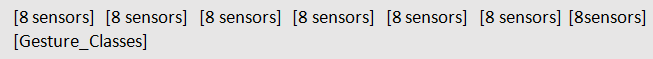
\includegraphics[scale=0.5]{Capture0.PNG}}
 \caption{Interface of of Data set}
  \label{fig:14}
\end{figure}
Data has been recorded at 200 Hz, meaning that every line is 8*(1/200) seconds = 40ms record time \cite{cve-2008-13689896464}. A class of gestures (0-3) determines when 64 figures are provided. Rock-0, Paper-1, Spherical-grip-2, Alright-3. Movements have been arbitrarily selected and amputees enrolled spontaneously have not faced any physical or mental issues in most cases. They has been embedded via the EMG (MayoWare) sensor and evaluated through the surface electrodes. Every activity has been reported with a gap of 6 periods for 20 seconds \cite{cve-2008-13689896464}. During every held organised movement, the tracking system was started. Although while still holding the movement, the tracking system was ceased. Motion takes a minimum of 120 seconds in a static position \cite{cve-2008-13689896464}. They all emerged from the same right forearm within a short period. The document has been merged in a .csv format with a name of (0-3) which has been presented at Table ~\ref{table:1}.
\begin{table}
\caption{Column Structure of Dataset}
\label{table:1}
\setlength{\tabcolsep}{3pt}
\begin{tabular}{|p{75pt}|p{25pt}|p{130pt}|}
 \hline
  Data \ Source & About \ This \ File & Columns \\
   \hline\hline
 	$0.csv$ \quad 65\;columns & muscle  &  \otimes  {+26.0} \ muscle \ reading \ 1 \ sensor \ 1 \\ 
 	 $1.csv$ \quad 65\;columns & activity & \otimes +04.0 \ muscle \ reading \ 1 \ sensor \ 2 \\ 
	 $2.csv$ \quad 65\;columns & while  & \otimes +05.0 \ muscle \ reading \ 1 \ sensor \ 3 \\ 
 	 $3.csv$ \quad 65\;columns & gesture \ 0  & \otimes +08.0 \ muscle \ reading \ 1 \ sensor \ 4 \\ 
     &  & \otimes -01.0 \ muscle \ reading \ 1 \ sensor \ 5 \\ 
     &  & \otimes -13.0 \ muscle \ reading \ 1 \ sensor \ 6 \\ 
     &  & \otimes -109.0 \ muscle \ reading \ 1 \ sensor \ 7 \\ 
     &  & \otimes -66.0 \ muscle \ reading \ 1 \ sensor \ 8 \\ 
\hline
\end{tabular}
\end{table}
\subsection{sEMG Signal Detection}
An accurate exposure of individual action in sEMG is an essential topic in the research of the hand’s motor system. A single-threshold system has been used to expose muscle timing on and off, analyzing the Root Mean Square (RMS) value of the reformed signals to thresholds whose result is based on the mean power of the framework of noise \cite{7428468}. The frequency range of the sEMG signal is (5-500) Hz. It requires frequency sampling greater than or equal to 1000Hz ~\cite{articlegfgf}. The limitations are up to  200  Hz  for  Myoware  Muscle  Sensor which has been used in this system. Reliable as well as effective methods such as noise refining, rectification, normalization etc. are needed to  process  the  collected  signals  accurately as  EMG data contains external and removable signals. Additionally, the amplitude ranges for the EMG signal before amplification is 0mV-10mV(5mV)~\cite{5234929}. As EMG signal is bipolar so it usually stretches both in positive and negative directions and tends to focus on zero as shown in Fig~\ref{fig:7}.
\begin{figure}[htbp]
 \centerline{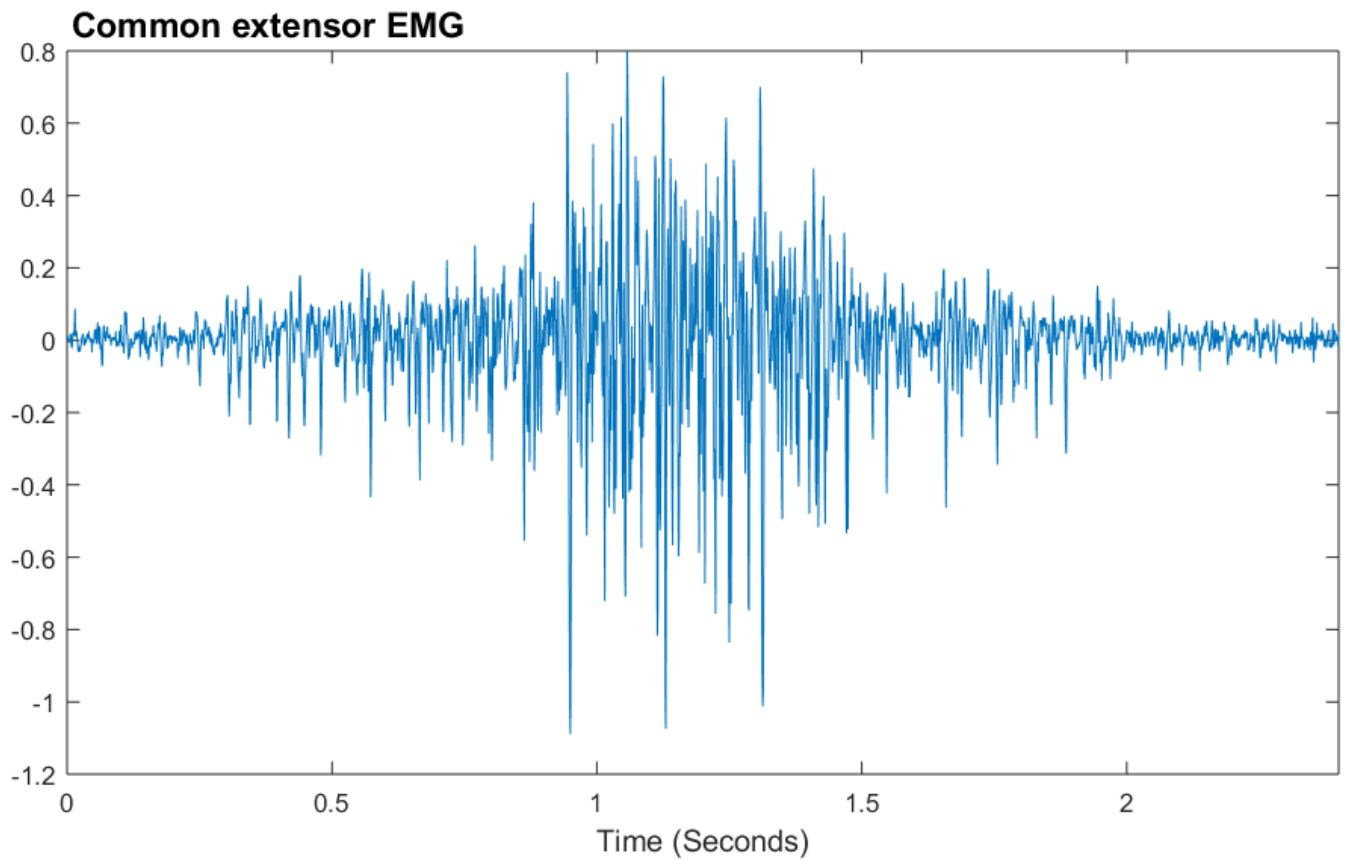
\includegraphics[scale=0.31]{fig7.JPG}}
 \caption{Nature of Raw EMG Sign}
  \label{fig:7}
\end{figure}\\
\subsection{SVM-KNN}
A difficult situation arises in deciding the kernel function parameters. In an attempt to find a solution for this problems, SVM has been combined with k-nearest neighbor classifier. It is the easy solution for deciding SVM kernel function parameter which reduces difficulty. SVM chooses only one optimized point from the plane where the hybrid algorithm chooses many for a single class. One class can hold many representative data points to represent a class in SVM-KNN. These facts can be observed in FIG~\ref{fig:8}. Maximum information gets exploited during the classification process. This system has an accuracy level of 95.398 \% which is approximate and higher than other algorithm approaches for classifying EMG data that is shown in  section \rom{7}.
\cite{article32}.
\begin{figure}[htbp]
 \centerline{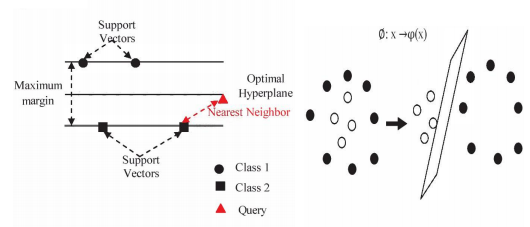
\includegraphics[scale=0.65]{Capture5.png}}
 \caption{SVM-KNN Classification}
  \label{fig:8}
\end{figure}\\
Support vector machine incorporating with the k-nearest neighbors has been developed where the classification depends solely on one phase of the sorted out class which also enumerates  the radial length of the groups characteristic. The screening approach is based on the support vector machine. While the reckoning threshold is smaller than the length, the exploited of the k-nearest neighbor algorithm would occur \cite{article32}. Explicit locality and scope have been used to distinguish the support vector among the observational units in the KNN algorithm \cite{article32}. K-nearest reference neighbor gets pinpointed where the exploratory elements gets separated. This leads to the enhancement of precision and the determination of the kernel framework for SVM \cite{article32}.
\
\section{Result and Analysis}
\subsection{KNN vs. SVM}
At first, the real live data has been acquired through signal of EMG. After that, pre-processing and feature extractions of signals have been executed that is acquired using different methods. Then, the data set has been classified in order to achieve the values for recognizing the motions as precise as possible. In the end, those achieved values has been implemented into to the simulation system and code instructions for acquiring the accuracy of each subject for each algorithm which has been presented through Table~\ref{table:7} and Table~\ref{table:8}. These are two of the existing concepts that has been being used to classify EMG patterns.
%%%%%%%%Table 7
\begin{table}

\caption{KNN standard classification accuracy rate}
			\centering
\begin{tabular}{p{0.32in}p{-0.01in}p{0.05in}p{0.05in}p{0.05in}p{0.05in}p{0.05in}p{0.05in}p{0.05in}p{-0.01in}p{0.11in}p{0.24in}}
\hline
%row no:1
\multicolumn{1}{|p{0.32in}}{{\fontsize{10pt}{12.0pt}\selectfont Data} \par {\fontsize{10pt}{12.0pt}\selectfont Sub}} &
\multicolumn{1}{|p{0.06in}}{{\fontsize{10pt}{12.0pt}\selectfont  1}} &
\multicolumn{1}{|p{0.06in}}{{\fontsize{10pt}{12.0pt}\selectfont  2}} &
\multicolumn{1}{|p{0.06in}}{{\fontsize{10pt}{12.0pt}\selectfont  3}} &
\multicolumn{1}{|p{0.06in}}{{\fontsize{10pt}{12.0pt}\selectfont  4}} &
\multicolumn{1}{|p{0.06in}}{{\fontsize{10pt}{12.0pt}\selectfont  5}} &
\multicolumn{1}{|p{0.06in}}{{\fontsize{10pt}{12.0pt}\selectfont  6}} &
\multicolumn{1}{|p{0.06in}}{{\fontsize{10pt}{12.0pt}\selectfont  7}} &
\multicolumn{1}{|p{0.06in}}{{\fontsize{10pt}{12.0pt}\selectfont  8}} &
\multicolumn{1}{|p{0.06in}}{{\fontsize{10pt}{12.0pt}\selectfont  9}} &
\multicolumn{1}{|p{0.06in}}{{\fontsize{10pt}{12.0pt}\selectfont  10}} &
\multicolumn{1}{|p{0.24in}|}{{\fontsize{10pt}{12.0pt}\selectfont Avg. in $\%$ }} \\
\hline
%row no:2
\multicolumn{1}{|p{0.32in}}{{\fontsize{10pt}{12.0pt}\selectfont  1\textsuperscript{st} Sub}} &
\multicolumn{1}{|p{0.06in}}{{\fontsize{10pt}{12.0pt}\selectfont 82}} &
\multicolumn{1}{|p{0.06in}}{{\fontsize{10pt}{12.0pt}\selectfont 81}} &
\multicolumn{1}{|p{0.06in}}{{\fontsize{10pt}{12.0pt}\selectfont 91}} &
\multicolumn{1}{|p{0.06in}}{{\fontsize{10pt}{12.0pt}\selectfont 93}} &
\multicolumn{1}{|p{0.06in}}{{\fontsize{10pt}{12.0pt}\selectfont 81}} &
\multicolumn{1}{|p{0.06in}}{{\fontsize{10pt}{12.0pt}\selectfont 96}} &
\multicolumn{1}{|p{0.06in}}{{\fontsize{10pt}{12.0pt}\selectfont 92}} &
\multicolumn{1}{|p{0.06in}}{{\fontsize{10pt}{12.0pt}\selectfont 85}} &
\multicolumn{1}{|p{0.06in}}{{\fontsize{10pt}{12.0pt}\selectfont 79}} &
\multicolumn{1}{|p{0.06in}}{{\fontsize{10pt}{12.0pt}\selectfont 88}} &
\multicolumn{1}{|p{0.06in}|}{{\fontsize{10pt}{12.0pt}\selectfont 86.80}} \\
\hline
%row no:3
\multicolumn{1}{|p{0.32in}}{{\fontsize{10pt}{12.0pt}\selectfont  2\textsuperscript{nd} Sub}} &
\multicolumn{1}{|p{0.06in}}{{\fontsize{10pt}{12.0pt}\selectfont 79}} &
\multicolumn{1}{|p{0.06in}}{{\fontsize{10pt}{12.0pt}\selectfont 93}} &
\multicolumn{1}{|p{0.06in}}{{\fontsize{10pt}{12.0pt}\selectfont 93}} &
\multicolumn{1}{|p{0.06in}}{{\fontsize{10pt}{12.0pt}\selectfont 93}} &
\multicolumn{1}{|p{0.06in}}{{\fontsize{10pt}{12.0pt}\selectfont 85}} &
\multicolumn{1}{|p{0.06in}}{{\fontsize{10pt}{12.0pt}\selectfont 80}} &
\multicolumn{1}{|p{0.06in}}{{\fontsize{10pt}{12.0pt}\selectfont 86}} &
\multicolumn{1}{|p{0.06in}}{{\fontsize{10pt}{12.0pt}\selectfont 90}} &
\multicolumn{1}{|p{0.06in}}{{\fontsize{10pt}{12.0pt}\selectfont 74}} &
\multicolumn{1}{|p{0.06in}}{{\fontsize{10pt}{12.0pt}\selectfont 77}} &
\multicolumn{1}{|p{0.24in}|}{{\fontsize{10pt}{12.0pt}\selectfont 85.00}} \\
\hline
%row no:4
\multicolumn{1}{|p{0.32in}}{{\fontsize{10pt}{12.0pt}\selectfont  3\textsuperscript{rd} Sub}} &
\multicolumn{1}{|p{0.06in}}{{\fontsize{10pt}{12.0pt}\selectfont 96}} &
\multicolumn{1}{|p{0.06in}}{{\fontsize{10pt}{12.0pt}\selectfont 87}} &
\multicolumn{1}{|p{0.06in}}{{\fontsize{10pt}{12.0pt}\selectfont 86}} &
\multicolumn{1}{|p{0.06in}}{{\fontsize{10pt}{12.0pt}\selectfont 72}} &
\multicolumn{1}{|p{0.06in}}{{\fontsize{10pt}{12.0pt}\selectfont 88}} &
\multicolumn{1}{|p{0.06in}}{{\fontsize{10pt}{12.0pt}\selectfont 93}} &
\multicolumn{1}{|p{0.06in}}{{\fontsize{10pt}{12.0pt}\selectfont 97}} &
\multicolumn{1}{|p{0.06in}}{{\fontsize{10pt}{12.0pt}\selectfont 79}} &
\multicolumn{1}{|p{0.06in}}{{\fontsize{10pt}{12.0pt}\selectfont 89}} &
\multicolumn{1}{|p{0.06in}}{{\fontsize{10pt}{12.0pt}\selectfont 88}} &
\multicolumn{1}{|p{0.24in}|}{{\fontsize{10pt}{12.0pt}\selectfont 87.50}} \\
\hline
%row no:5
\multicolumn{1}{|p{0.32in}}{{\fontsize{10pt}{12.0pt}\selectfont  4\textsuperscript{th} Sub}} &
\multicolumn{1}{|p{0.06in}}{{\fontsize{10pt}{12.0pt}\selectfont 96}} &
\multicolumn{1}{|p{0.12in}}{{\fontsize{10pt}{12.0pt}\selectfont 100}} &
\multicolumn{1}{|p{0.06in}}{{\fontsize{10pt}{12.0pt}\selectfont 92}} &
\multicolumn{1}{|p{0.13in}}{{\fontsize{10pt}{12.0pt}\selectfont 92}} &
\multicolumn{1}{|p{0.06in}}{{\fontsize{10pt}{12.0pt}\selectfont 84}} &
\multicolumn{1}{|p{0.06in}}{{\fontsize{10pt}{12.0pt}\selectfont 95}} &
\multicolumn{1}{|p{0.06in}}{{\fontsize{10pt}{12.0pt}\selectfont 85}} &
\multicolumn{1}{|p{0.06in}}{{\fontsize{10pt}{12.0pt}\selectfont 93}} &
\multicolumn{1}{|p{0.06in}}{{\fontsize{10pt}{12.0pt}\selectfont 97}} &
\multicolumn{1}{|p{0.06in}}{{\fontsize{10pt}{12.0pt}\selectfont 88}} &
\multicolumn{1}{|p{0.24in}|}{{\fontsize{10pt}{12.0pt}\selectfont 92.20 }} \\
\hline
%row no:6
\multicolumn{1}{|p{0.32in}}{{\fontsize{10pt}{12.0pt}\selectfont  5\textsuperscript{th} Sub}} &
\multicolumn{1}{|p{0.06in}}{{\fontsize{10pt}{12.0pt}\selectfont 90}} &
\multicolumn{1}{|p{0.06in}}{{\fontsize{10pt}{12.0pt}\selectfont 84}} &
\multicolumn{1}{|p{0.06in}}{{\fontsize{10pt}{12.0pt}\selectfont 92}} &
\multicolumn{1}{|p{0.06in}}{{\fontsize{10pt}{12.0pt}\selectfont 95}} &
\multicolumn{1}{|p{0.06in}}{{\fontsize{10pt}{12.0pt}\selectfont 95}} &
\multicolumn{1}{|p{0.06in}}{{\fontsize{10pt}{12.0pt}\selectfont 90}} &
\multicolumn{1}{|p{0.06in}}{{\fontsize{10pt}{12.0pt}\selectfont 90}} &
\multicolumn{1}{|p{0.06in}}{{\fontsize{10pt}{12.0pt}\selectfont 96}} &
\multicolumn{1}{|p{0.06in}}{{\fontsize{10pt}{12.0pt}\selectfont 89}} &
\multicolumn{1}{|p{0.06in}}{{\fontsize{10pt}{12.0pt}\selectfont 93}} &
\multicolumn{1}{|p{0.24in}|}{{\fontsize{10pt}{12.0pt}\selectfont 91.40}} \\
\hline
%row no:7
\multicolumn{1}{|p{0.32in}}{} &
\multicolumn{1}{|p{0.06in}}{} &
\multicolumn{1}{|p{0.06in}}{} &
\multicolumn{1}{|p{0.06in}}{} &
\multicolumn{1}{|p{0.06in}}{} &
\multicolumn{1}{|p{0.06in}}{} &
\multicolumn{1}{|p{0.06in}}{} &
\multicolumn{1}{|p{0.06in}}{} &
\multicolumn{1}{|p{0.06in}}{} &
\multicolumn{1}{|p{0.06in}}{} &
\multicolumn{1}{|p{0.11in}}{{\fontsize{10pt}{12.0pt}\selectfont Av.}} &
\multicolumn{1}{|p{0.24in}|}{{\fontsize{10pt}{12.0pt}\selectfont \textbf{88.58}}} \\
\hline
\label{table:7}
\end{tabular}
 \end{table}

%%%%%%%%%Table SVM Start%%%%%%%%%
\begin{table}
\label{table:8}
\caption{SVM standard classification accuracy rate}
			\centering
\begin{tabular}{p{0.32in}p{-0.01in}p{0.05in}p{0.05in}p{0.05in}p{0.05in}p{0.05in}p{0.05in}p{0.05in}p{-0.01in}p{0.11in}p{0.24in}}
\hline
%row no:1
\multicolumn{1}{|p{0.32in}}{{\fontsize{10pt}{12.0pt}\selectfont Data} \par {\fontsize{10pt}{12.0pt}\selectfont Sub}} &
\multicolumn{1}{|p{0.01in}}{{\fontsize{10pt}{12.0pt}\selectfont  1}} &
\multicolumn{1}{|p{0.01in}}{{\fontsize{10pt}{12.0pt}\selectfont  2}} &
\multicolumn{1}{|p{0.01in}}{{\fontsize{10pt}{12.0pt}\selectfont  3}} &
\multicolumn{1}{|p{0.01in}}{{\fontsize{10pt}{12.0pt}\selectfont  4}} &
\multicolumn{1}{|p{0.01in}}{{\fontsize{10pt}{12.0pt}\selectfont  5}} &
\multicolumn{1}{|p{0.01in}}{{\fontsize{10pt}{12.0pt}\selectfont  6}} &
\multicolumn{1}{|p{0.01in}}{{\fontsize{10pt}{12.0pt}\selectfont  7}} &
\multicolumn{1}{|p{0.01in}}{{\fontsize{10pt}{12.0pt}\selectfont  8}} &
\multicolumn{1}{|p{-0.01in}}{{\fontsize{10pt}{12.0pt}\selectfont  9}} &
\multicolumn{1}{|p{0.11in}}{{\fontsize{10pt}{12.0pt}\selectfont  10}} &
\multicolumn{1}{|p{0.24in}|}{{\fontsize{10pt}{12.0pt}\selectfont Avg. in $\%$ }} \\
\hline
%row no:2
\multicolumn{1}{|p{0.32in}}{{\fontsize{10pt}{12.0pt}\selectfont  1\textsuperscript{st} Sub}} &
\multicolumn{1}{|p{0.06in}}{{\fontsize{10pt}{12.0pt}\selectfont 98}} &
\multicolumn{1}{|p{0.06in}}{{\fontsize{10pt}{12.0pt}\selectfont 86}} &
\multicolumn{1}{|p{0.06in}}{{\fontsize{10pt}{12.0pt}\selectfont 95}} &
\multicolumn{1}{|p{0.06in}}{{\fontsize{10pt}{12.0pt}\selectfont 83}} &
\multicolumn{1}{|p{0.06in}}{{\fontsize{10pt}{12.0pt}\selectfont 83}} &
\multicolumn{1}{|p{0.06in}}{{\fontsize{10pt}{12.0pt}\selectfont 91}} &
\multicolumn{1}{|p{0.06in}}{{\fontsize{10pt}{12.0pt}\selectfont  89}} &
\multicolumn{1}{|p{0.06in}}{{\fontsize{10pt}{12.0pt}\selectfont  97}} &
\multicolumn{1}{|p{0.06in}}{{\fontsize{10pt}{12.0pt}\selectfont 97}} &
\multicolumn{1}{|p{0.06in}}{{\fontsize{10pt}{12.0pt}\selectfont 86}} &
\multicolumn{1}{|p{0.24in}|}{{\fontsize{10pt}{12.0pt}\selectfont 90.50}} \\
\hline
%row no:3
\multicolumn{1}{|p{0.32in}}{{\fontsize{10pt}{12.0pt}\selectfont  2\textsuperscript{nd} Sub}} &
\multicolumn{1}{|p{0.06in}}{{\fontsize{10pt}{12.0pt}\selectfont 96}} &
\multicolumn{1}{|p{0.06in}}{{\fontsize{10pt}{12.0pt}\selectfont 96}} &
\multicolumn{1}{|p{0.06in}}{{\fontsize{10pt}{12.0pt}\selectfont 95}} &
\multicolumn{1}{|p{0.06in}}{{\fontsize{10pt}{12.0pt}\selectfont 93}} &
\multicolumn{1}{|p{0.06in}}{{\fontsize{10pt}{12.0pt}\selectfont 83}} &
\multicolumn{1}{|p{0.06in}}{{\fontsize{10pt}{12.0pt}\selectfont 88}} &
\multicolumn{1}{|p{0.06in}}{{\fontsize{10pt}{12.0pt}\selectfont 96}} &
\multicolumn{1}{|p{0.06in}}{{\fontsize{10pt}{12.0pt}\selectfont  96}} &
\multicolumn{1}{|p{0.06in}}{{\fontsize{10pt}{12.0pt}\selectfont 88}} &
\multicolumn{1}{|p{0.06in}}{{\fontsize{10pt}{12.0pt}\selectfont  84}} &
\multicolumn{1}{|p{0.24in}|}{{\fontsize{10pt}{12.0pt}\selectfont 91.50}} \\
\hline
%row no:4
\multicolumn{1}{|p{0.32in}}{{\fontsize{10pt}{12.0pt}\selectfont  3\textsuperscript{rd} Sub}} &
\multicolumn{1}{|p{0.06in}}{{\fontsize{10pt}{12.0pt}\selectfont 98}} &
\multicolumn{1}{|p{0.06in}}{{\fontsize{10pt}{12.0pt}\selectfont 89}} &
\multicolumn{1}{|p{0.12in}}{{\fontsize{10pt}{12.0pt}\selectfont 88}} &
\multicolumn{1}{|p{0.12in}}{{\fontsize{10pt}{12.0pt}\selectfont 100}} &
\multicolumn{1}{|p{0.06in}}{{\fontsize{10pt}{12.0pt}\selectfont 97}} &
\multicolumn{1}{|p{0.06in}}{{\fontsize{10pt}{12.0pt}\selectfont 97}} &
\multicolumn{1}{|p{0.06in}}{{\fontsize{10pt}{12.0pt}\selectfont 97}} &
\multicolumn{1}{|p{0.06in}}{{\fontsize{10pt}{12.0pt}\selectfont  94}} &
\multicolumn{1}{|p{0.06in}}{{\fontsize{10pt}{12.0pt}\selectfont 94}} &
\multicolumn{1}{|p{0.06in}}{{\fontsize{10pt}{12.0pt}\selectfont  88}} &
\multicolumn{1}{|p{0.24in}|}{{\fontsize{10pt}{12.0pt}\selectfont 90.90}} \\
\hline
%row no:5
\multicolumn{1}{|p{0.32in}}{{\fontsize{10pt}{12.0pt}\selectfont  4\textsuperscript{th} Sub}} &
\multicolumn{1}{|p{0.06in}}{{\fontsize{10pt}{12.0pt}\selectfont 87}} &
\multicolumn{1}{|p{0.06in}}{{\fontsize{10pt}{12.0pt}\selectfont 90}} &
\multicolumn{1}{|p{0.06in}}{{\fontsize{10pt}{12.0pt}\selectfont 94}} &
\multicolumn{1}{|p{0.06in}}{{\fontsize{10pt}{12.0pt}\selectfont 95}} &
\multicolumn{1}{|p{0.06in}}{{\fontsize{10pt}{12.0pt}\selectfont  95}} &
\multicolumn{1}{|p{0.06in}}{{\fontsize{10pt}{12.0pt}\selectfont 95}} &
\multicolumn{1}{|p{0.06in}}{{\fontsize{10pt}{12.0pt}\selectfont 95}} &
\multicolumn{1}{|p{0.06in}}{{\fontsize{10pt}{12.0pt}\selectfont  89}} &
\multicolumn{1}{|p{0.06in}}{{\fontsize{10pt}{12.0pt}\selectfont 89}} &
\multicolumn{1}{|p{0.12in}}{{\fontsize{10pt}{12.0pt}\selectfont  100}} &
\multicolumn{1}{|p{0.24in}|}{{\fontsize{10pt}{12.0pt}\selectfont 92.90}} \\
\hline
%row no:6
\multicolumn{1}{|p{0.32in}}{{\fontsize{10pt}{12.0pt}\selectfont  5\textsuperscript{th} Sub}} &
\multicolumn{1}{|p{0.06in}}{{\fontsize{10pt}{12.0pt}\selectfont 90}} &
\multicolumn{1}{|p{0.06in}}{{\fontsize{10pt}{12.0pt}\selectfont 91}} &
\multicolumn{1}{|p{0.06in}}{{\fontsize{10pt}{12.0pt}\selectfont 91}} &
\multicolumn{1}{|p{0.06in}}{{\fontsize{10pt}{12.0pt}\selectfont 91}} &
\multicolumn{1}{|p{0.06in}}{{\fontsize{10pt}{12.0pt}\selectfont  95}} &
\multicolumn{1}{|p{0.06in}}{{\fontsize{10pt}{12.0pt}\selectfont 88}} &
\multicolumn{1}{|p{0.06in}}{{\fontsize{10pt}{12.0pt}\selectfont  92}} &
\multicolumn{1}{|p{0.12in}}{{\fontsize{10pt}{12.0pt}\selectfont 99}} &
\multicolumn{1}{|p{0.06in}}{{\fontsize{10pt}{12.0pt}\selectfont 86}} &
\multicolumn{1}{|p{0.06in}}{{\fontsize{10pt}{12.0pt}\selectfont  98}} &
\multicolumn{1}{|p{0.24in}|}{{\fontsize{10pt}{12.0pt}\selectfont 92.10}} \\
\hline
%row no:7
\multicolumn{1}{|p{0.32in}}{} &
\multicolumn{1}{|p{0.06in}}{} &
\multicolumn{1}{|p{0.06in}}{} &
\multicolumn{1}{|p{0.06in}}{} &
\multicolumn{1}{|p{0.06in}}{} &
\multicolumn{1}{|p{0.06in}}{} &
\multicolumn{1}{|p{0.06in}}{} &
\multicolumn{1}{|p{0.06in}}{} &
\multicolumn{1}{|p{0.06in}}{} &
\multicolumn{1}{|p{0.06in}}{} &
\multicolumn{1}{|p{0.06in}}{{\fontsize{10pt}{12.0pt}\selectfont Av.}} &
\multicolumn{1}{|p{0.24in}|}{{\fontsize{10pt}{12.0pt}\selectfont \textbf{92.24}}} \\
\hline

\end{tabular}
\label{table:8}
 \end{table}
%%%%%%%%%Table SVM end%%%%%%%%%

\subsection{AVERAGE CATEGORIZATION RATE } 
The Fig~\ref{fig:29} describes the overall categorization score for all subjects that is \textbf{95.398\%} for using the hybrid algorithm which is the mixture of SVM and KNN. The accuracy is greater than using only SVM or using only KNN. Fig~\ref{fig:29} illustrates an average value of categorization for individual subject wherein the x-axis indicates a particular subject and each measurement has been defined in conjunction with the individual subject and vertical column which is in y-axis, reflecting a generalized average rate of categorization. Same method of implementing the user values to the simulation system and code instructions which was done in SVM and KNN has been used in acquiring accuracy related data for SVM-KNN hybrid algorithm.
\begin{figure}[htbp]
 \centerline{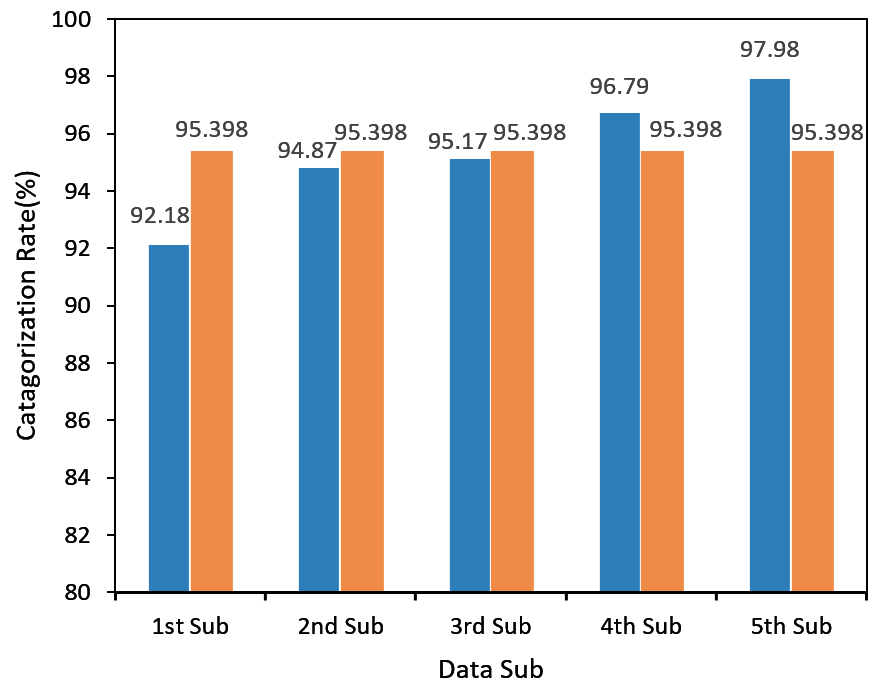
\includegraphics[scale=0.5]{ne dhappa 2.PNG}}
 \caption{Accuracy of different subjects using hybrid algorithm (SVM-KNN)}
  \label{fig:29}
\end{figure} 

\newpage
\section{Conclusion}
To conclude, people are losing their body parts daily in developing countries like
Bangladesh. The reason behind this leads to huge road accidents, tracking, diseases like diabetes etc. This kind of amputee people need prosthesis so that they can make their life a little easier. As the costs of Bionic robotic parts are so high, the system has proposed a model where sEMG controlled recordings have been used in training system model. It is very precise as well as affordable system for most of the amputees which can make their life easier.\\


\bibliography{biblio.bib}
\bibliographystyle{unsrt}


\end{document}
